\documentclass[10pt,openany,oneside]{book}
\usepackage{geometry, graphicx, floatflt, varioref, soul, verbatim, amsmath, calc, caption, wasysym, footmisc, makeidx, ifthen, subfigure, multicol, epstopdf, enumerate, wrapfig, textcomp, multirow, changepage, setspace, lscape}
\usepackage[numbers]{natbib}
\usepackage[usenames,dvipsnames]{color}      

\definecolor{oiGA}{rgb}{0,0,0}
\definecolor{oiGB}{rgb}{.5,.5,.5}
\definecolor{oiGC}{rgb}{.85,.85,.85}
\definecolor{oiB}{rgb}{.337,.608,.741}
\definecolor{oiG}{rgb}{.298,.447,.114}
\definecolor{oiY}{rgb}{.957,.863,0}
\definecolor{oiR}{rgb}{.941,.318,.200}
\definecolor{redcards}{rgb}{.941,.318,.200}


\definecolor{rd}{rgb}{.80,.0,.0}
\definecolor{tableHL}{rgb}{.5,.1,.2}
\definecolor{tableHLBlue}{rgb}{.2,.4,.9}
\definecolor{highlight}{rgb}{.5,.1,.2}
\definecolor{highlightO}{rgb}{.1,.3,.8}
\definecolor{highlightT}{rgb}{.6,.3,.1}
\definecolor{ex}{rgb}{.0,.30,.55}
\definecolor{gray}{rgb}{.5,.5,.5}
\definecolor{steelBlue}{rgb}{.3,.4,.8}
\definecolor{excolor}{rgb}{.0,.3,.55}
\definecolor{secolor}{rgb}{.0,.3,.55}
\definecolor{comment}{rgb}{.65,.45,.25}
\definecolor{grayDark}{rgb}{.43,.43,.43}
\definecolor{grayLight}{rgb}{.65,.65,.65}
\definecolor{examplegray}{rgb}{0,0,0} %{.83,.83,.83}
\definecolor{termOColor}{rgb}{.65,.1,.1}

 
%\newcommand{\href}[2]{#2} \newcommand{\url}[1]{#1} \newcommand{\urlstyle}[1]{}
\usepackage[colorlinks=false,pdfborder={0 0 0},urlcolor= oiGB,colorlinks=true,linkcolor= oiGB, citecolor= oiGB,backref=true]{hyperref}
%\usepackage[colorlinks=false,pdfborder={0 0 0},urlcolor= MidnightBlue,colorlinks=false,linkcolor= MidnightBlue, citecolor= MidnightBlue,backref=true]{hyperref}
%\usepackage{ifsym}
%\usepackage{fancybox}

\makeindex
% 1 Page Parameters
% 2 Special Commands for Editions
% 3 Content Modifications
% 4 Counters and Parameters
% 5 Section Coloring
% 6 Utilities
% 7 
% 8 Figures and Captions
% 9 Examples and Exercises
% 10 Special Boxes




%-------------------------------------------------------------
% 1 Page Parameters
% 1.1 Amazon
\setlength\paperheight{10in}
\setlength\textheight{8.25in}
\setlength\paperwidth{8in}
\setlength\textwidth{5.45in}
\setlength\voffset{-10mm}
% 1.2 Margin Size
% 1.2.1 Slim
%\setlength\hoffset{0.25in}
%\setlength\oddsidemargin{0.25in}
%\setlength\evensidemargin{0in}
% 1.2.2 Medium
\setlength\hoffset{3.7mm}
\setlength\oddsidemargin{3mm}
\setlength\evensidemargin{3mm}
% 1.2.3 Wide
%\setlength\hoffset{-5mm}
%\setlength\oddsidemargin{0.5in}
%\setlength\evensidemargin{0.5in}
% 1.3 PDF Parameters
%\setlength\paperheight{11in}
%\setlength\textheight{8.25in}
%\setlength\paperwidth{8.5in}
%\setlength\textwidth{5.45in}
%\setlength\voffset{-10mm}
%\setlength\oddsidemargin{0.75in}
%\setlength\evensidemargin{0.75in}
% 1.4 Margin Spacing
\setlength{\marginparsep}{5mm}
\setlength{\marginparwidth}{20mm}




%-------------------------------------------------------------
% 2 Special Commands for Editions
\newcommand{\vspaceB}[1]{\vspace{#1}}
\newcommand{\hspaceB}[1]{\hspace{#1}}
\newcommand{\textB}[1]{#1}



%-------------------------------------------------------------
% 3 Content Modifications
\newcommand{\APVersion}[2]{#2}
\newcommand{\MultipleRegression}[2]{#1}
\newcommand{\MultipleRegressionChapter}[2]{#1}
\newcommand{\SimulationAndRandomization}[1]{#1}
\newcommand{\ANOVASection}[2]{#1}
\newcommand{\GLMSection}[2]{#1}




%-------------------------------------------------------------
% 4 Counters and Parameters
% 4.1 Counters
\newcounter{alwaysOne}
\setcounter{alwaysOne}{1}
\newcounter{alwaysTwo}
\setcounter{alwaysTwo}{2}
\newcounter{alwaysThree}
\setcounter{alwaysThree}{3}
\newcounter{alwaysFour}
\setcounter{alwaysFour}{4}
\newcounter{withinChNum}[chapter]
\setcounter{withinChNum}{0}
\newcounter{eoce}[chapter]
\renewcommand{\theeoce}{\arabic{chapter}.\arabic{eoce}}
\newcounter{eocesolch}
\setcounter{eocesolch}{0}
\newcounter{eocesol}[eocesolch]
% 4.2 Parameters
\newlength{\exampleAboveBar}
\newlength{\exampleBelowBar}
\setlength{\exampleAboveBar}{-3.15mm}
\setlength{\exampleBelowBar}{-1.15mm}




%%-------------------------------------------------------------
%% 5 Section Coloring
%% 5.1 Chapter
%\titleformat{\chapter}[display]
%{\color{oiB}\normalfont\huge\bfseries\raggedright}{\chaptertitlename\
%\thechapter}{20pt}{\Huge}
% 5.2 Section
\renewcommand{\thesection}{\arabic{section}}
%\titleformat{\section}
%{\color{oiB}\normalfont\Large\bfseries}
%{\color{oiB}\thesection}{1em}{}
% 5.3 Subsection
\renewcommand{\thesubsection}{%\arabic{section}.
\arabic{subsection}}
%\titleformat{\subsection}
%{\color{oiB}\normalfont\large\bfseries}
%{\color{oiB}\thesubsection}{1em}{}


%-------------------------------------------------------------
% 6 Utilities
% 6.1 Helpful Editing Commands
\newcommand\Add[1]{\marginpar[\color{oiR}$\bullet$]{\color{oiR}$\bullet$}{\color{oiB}#1}}
\newcommand\Cut[1]{\marginpar[\color{oiR}$\bullet$]{\color{oiR}$\bullet$}{\color{oiGC}#1}}
\newcommand\Comment[1]{\marginpar[\color{oiR}$\bullet$]{\color{oiR}$\bullet$} {\color{oiG}{[#1]}}}
\newcommand{\note}[1]{\Comment{#1}}
% 6.2 Special Symbols
\newcommand{\degree}{\ensuremath{^\circ}}
% 6.3 Text Commands (Terms, Data, Variable, Response)
\newcommand{\term}[1]{\textbf{#1}\index{#1|textbf}}
\newcommand{\termsub}[2]{\textbf{#1}\index{#2|textbf}}
\newcommand{\termni}[1]{\textbf{#1}}
\newcommand{\hiddenterm}[1]{#1\index{#1|textbf}}
\newcommand{\indexthis}[2]{#1\index{#2}}
\newcommand{\termO}[1]{\textbf{\color{termOColor}#1}}
\newenvironment{data}[1]{\texttt{#1}}{}
\newenvironment{var}[1]{\texttt{#1}}{}
\newenvironment{resp}[1]{\texttt{#1}}{}
% 6.4 Highlighting
\newenvironment{highlight}{\textbf}{}
\newcommand{\highlightO}[1]{\textbf{\color{oiB}#1}}
\newcommand{\highlightT}[1]{\emph{\color{oiR}#1}}
% 6.5 Lengths
\setlength{\parindent}{0.3in}
% 6.6 Hyperreferences
\newcommand{\urlwofont}[1]{\urlstyle{same}\url{#1}}



%-------------------------------------------------------------
% 7 



%-------------------------------------------------------------
% 8 Figures and Captions
% 8.1 Table Caption
\DeclareCaptionFormat{nbTab}{Table\nobreakspace\refstepcounter{withinChNum}\setcounter{table}{\value{withinChNum}}\setcounter{figure}{\value{withinChNum}}\thewithinChNum:\nobreakspace#3}
\captionsetup[table]{format=nbTab}
% 8.2 Figure Caption
\DeclareCaptionFormat{nbFig}{Figure\nobreakspace\refstepcounter{withinChNum}\setcounter{table}{\value{withinChNum}}\setcounter{figure}{\value{withinChNum}}\thewithinChNum:\nobreakspace#3}
\captionsetup[figure]{format=nbFig}
% 8.3 Caption Width
\newlength{\mycaptionwidth}
\setlength{\mycaptionwidth}{0.825\textwidth}
\setlength{\captionwidth}{\mycaptionwidth}




%-------------------------------------------------------------
% 9 Examples and Exercises
% 9.1 Exercises, within the text
% 9.1.1 Exercise Environment
\newcommand{\excolor}[1]{{\color{excolor}#1}}
\newenvironment{exercise}
{
\begin{itemize}\item[\color{oiB}$\bigodot$]\refstepcounter{equation}\noindent\normalsize\textbf{\color{oiB}Exercise \theexercise}\hspace{3mm}}
{\normalsize

\addvspace{3mm}
\end{itemize}}
% 9.1.2 Exercise Fine Tuning
\newcommand\theexercise{\arabic{equation}}
% 9.2 Examples
% 9.2.1 Example Environment
\newcommand\theexample{\arabic{equation}}
\newenvironment{example}[1]
{\begin{itemize}
\item[\color{oiB}\Large$\CIRCLE$]\refstepcounter{equation}\noindent\textbf{\color{oiB}Example \theexample}\hspace{0.3cm}#1\vspace{\exampleAboveBar}

{\color{examplegray}\rule{20mm}{0.1mm}}

\vspace{\exampleBelowBar}

\normalsize}{

\end{itemize}
\addvspace{3mm}
}
% 9.3 EOCEs: End of Chapter Exercises
% 9.3.1 Environment
\newenvironment{eoce}[2]
{\refstepcounter{eoce}\noindent\small\textbf{\textcolor{oiB}{\arabic{chapter}.\arabic{eoce}}}\hspace{2mm} #1

\addvspace{3mm}

}
%{\em #2 } $\:$ \\ }
{}
% 9.3.2 EOCE Solutions
\newcommand{\eocesolch}[1]{
\refstepcounter{eocesolch}\noindent\textbf{\color{oiB}\arabic{eocesolch}\hspace{2mm}#1}

\addvspace{2mm}

}
\newcommand{\eocesol}[1]{\refstepcounter{eocesol}\noindent\textbf{\color{oiB}\arabic{eocesolch}.\arabic{eocesol}}\hspace{2mm}{\small#1}\addtocounter{eocesol}{1}

\addvspace{1mm}

}
% 9.3.3 EOCE Utilities
\newcommand{\qt}[1]{\textcolor{oiB}{\textbf{#1.}}}
\newcommand{\qtq}[1]{\textcolor{oiB}{\textbf{#1?}}}
\newcommand{\ec}[1]{\textcolor{oiB}{\footnotesize{~(#1)}}}% 9.3.4 EOCE Roman Parts
\newenvironment{romanparts}{
\begin{enumerate}[I.]
\setlength{\itemsep}{0mm}
}{\end{enumerate}}
% 9.3.5 EOCE Parts
\newenvironment{parts}{
%\vspace{-0.25cm}
\begin{enumerate}[(a)]
\setlength{\itemsep}{0mm}}
{\end{enumerate}}
% 9.3.6 EOCE Subparts
\newenvironment{subparts}{
\begin{enumerate}[i.]
\setlength{\itemsep}{0mm}}
{\end{enumerate}}
% 9.3.7 EOCE hyp environment
\newenvironment{hyp}{
\begin{itemize}
\setlength{\itemsep}{0mm}
}
{\end{itemize}
}
% 9.3.8 cond environment
\newenvironment{cond}{
\begin{enumerate}[1.]
\setlength{\itemsep}{0mm}
}
{\end{enumerate}
}




%-------------------------------------------------------------
% 10 Special Boxes
% 10.1 Term Box
\newenvironment{tBoxTitle}[2][\\]{\textbf{\color{oiB}#2} #1
}{}
\newenvironment{termBox}[1]{
\addvspace{4mm}
\noindent{\color{oiB}\framebox[\textwidth][c]{\framebox[\textwidth-3mm][l]{ \\
	\vspace{0.5cm} \\
	\begin{minipage}[b]{\textwidth-3mm}
		\begin{minipage}[t]{2mm}
			\hspace{2mm}
		\end{minipage}
		\begin{minipage}[b]{\textwidth-10mm}
			\color{black}#1
		\end{minipage}
	\end{minipage}}}}
}{

\addvspace{1mm}}
% 10.2 Tip Box
\newenvironment{tipBoxTitle}[2][TIP:\ ]{\textbf{\color{oiB}#1#2} \\
}{}
\newenvironment{tipBox}[1]{
\addvspace{4mm}
\noindent{\color{oiB}\framebox[\textwidth][l]{ \\
	\vspace{5mm} \\
	\begin{minipage}[b]{\textwidth-4mm}
		\begin{minipage}[t]{2mm}
			\hspace{2mm}
		\end{minipage}
		\begin{minipage}[b]{\textwidth-8mm}
			\color{black}#1
		\end{minipage}
	\end{minipage}}}
}{

\addvspace{1mm}}
% 10.3 Caution Box
\newenvironment{caution}[2]{
\addvspace{4mm}
\noindent{\color{oiB}\framebox[\textwidth][l]{ \\
	\vspace{5mm} \\
	\begin{minipage}[b]{\textwidth-4mm}
		\begin{minipage}[t]{2mm}
			\hspace{2mm}
		\end{minipage}
		\begin{minipage}[b]{\textwidth-8mm}
			\textbf{\color{oiB}Caution: #1} \\
			\color{black}#2
		\end{minipage}
	\end{minipage}}}
}{

\addvspace{1mm}}







\date{}
\begin{document}

\section*{OpenIntro online supplement}

This material is an online resource of OpenIntro textbooks, which are available for free in PDF at \href{http://www.openintro.org/books}{openintro.org/books} and also sold at affordable prices in paperback and hardcover. This supplement is licensed under a Creative Commons license, and you are welcome to share it with others. For additional details on the license this document is under, see \href{http://www.openintro.org/rights.php}{www.openintro.org/rights.php}.

%
\section*{Weighted mean}

The weighted mean is the same as the mean, except that it is influenced more by some observations than others. We assign weights to observations as a sort of way of describing its relative importance. In many applications, there are natural choices for weights. For example, in the \data{county} data set, population is a natural weighting factor.

Given the number of people in each county of the United States and also the average income per person in each county, how should we compute the average income per person for residents in the United States?

An initial guess might ignore the population data. This would yield a mean income of about \$22,505. However, this is not the mean income of the people in the United States, which is actually several thousand dollars more. To see why, consider Figure~\ref{incomeVsPop}, which shows the income and population of all 3,143 counties. Notice first that the scale on the horizontal axis for population shows a special scale (called the log-scale). Many of the biggest counties have higher incomes than the smaller counties. This is why our original mean calculation gives a wrong answer.
\begin{figure}
\centering
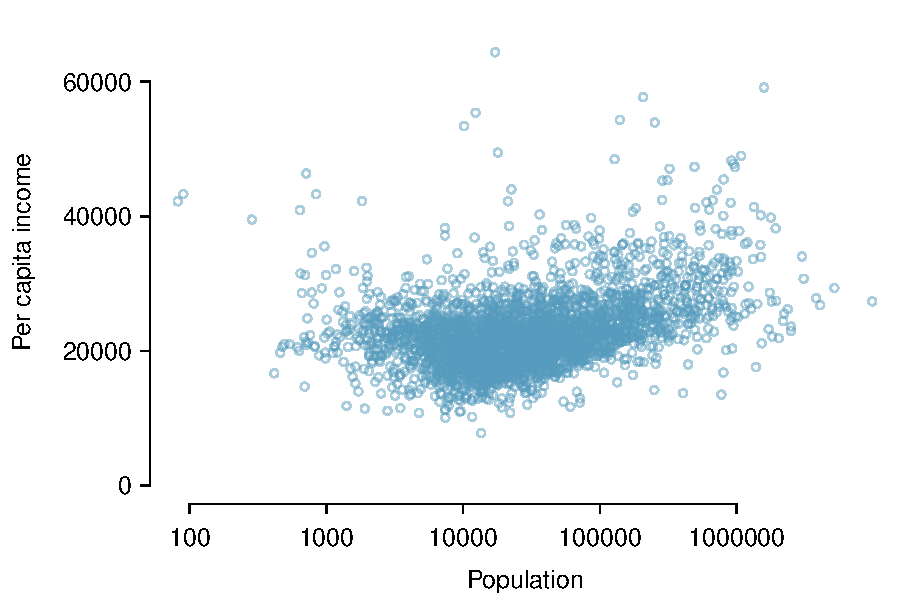
\includegraphics[width=\textwidth]{WeightedMean/figures/incomeVsPop/incomeVsPop} 
\caption{Per capita income against population size in 3,143 US counties.}
\label{incomeVsPop}
\end{figure}

Let's think again about the regular problem: we want the mean income per person in the United States. We need exactly two numbers to complete this calculation: the total income of all people in the US and the number of people in the US:
\begin{align*}
\frac{\text{Total income of all people in the US}}{\text{Number of people in the US}}
\end{align*}
We're not given these numbers, but the data provided is sufficient to calculate each of the numbers. Starting with the denominator (the bottom), just add up the population in all the counties: 308,745,538.

The numerator (the top of the fraction) is a little tougher, but not much. If we had the total income of all people each county, then we could add up all those values to get the total income. To get the income for any given county, we can multiple the average income of the county with the number of people in the county. This just relies on a rearrangement of the equation defining the average income for the county:
\begin{align*}
\text{Ave income} = \frac{\text{County income}}{\text{Num. people in county}}
\end{align*}
\begin{align*}
\Downarrow
\end{align*}
\begin{align*}
(\text{Ave income})(\text{Num. people in county}) = \text{County income}
\end{align*}
Now that we can get the county incomes, we can get the income for the entire United States: about \$8.4447 trillion (\$8,444,700 million). Finally, we can calculate the average income in the United States:
\begin{align*}
\frac{\text{Total income of all people in the US}}{\text{Number of people in the US}}
	= \frac{\text{\$8,444,700,000,000}}{\text{308,745,538}} = \$27,348
\end{align*}
Recall that the simple mean was \$22,505.

Let's put the entire calculation into a single expression. We'll use $w_1$ to represent the population of the first county, $w_2$ to represent the population of the second county, and so on. The label $x_1$ will represent the average income of county 1, $x_2$ for the average income of county 2, and so on. Then the mean weighted by population can be written as
\begin{align*}
\frac{w_{1}x_{1} + w_{2}x_{2} + w_{3}x_{3} + \dots + w_{3143}x_{3143}}
	{w_{1} + w_{2} + w_{3} + \dots + w_{3143}}
\end{align*}
This equation represents the \term{weighted mean} of income, where the weights are given by the population values.

\begin{termBox}{\tBoxTitle{Weighted mean}
The weighed mean of observations $x_1$, $x_2$, ..., $x_n$ using weights $w_1$, $w_2$, ..., $w_n$ is given by
\begin{align*}
\text{weighted mean of $x_i$s} = 
\frac{w_{1}x_{1} + w_{2}x_{2} + \dots + w_{n}x_{n}}
	{w_{1} + w_{2} + \dots + w_{n}} = 
\frac{\sum_{i=1}^n w_{i}x_{i}}
	{\sum_{i=1}^n w_{i}}
\end{align*}
If the second equation with the $\Sigma$s isn't math notation you feel comfortable with, just consider the first definition. The second expression is just a fancy way of making the equation compact.}\end{termBox}

\begin{tipBox}{\tipBoxTitle{Simple mean is a special case of the weighted mean}
The simple mean is a weighted mean where all the weights are~1:
\begin{align*}
\frac{x_{1} + x_{2} + x_{3} + \dots + x_{n}}
	{n}
= \frac{1\times x_{1} + 1\times x_{2} + 1\times x_{3} + \dots + 1\times x_{n}}
	{1 + 1 + 1 + \dots + 1}
\end{align*}
}\end{tipBox}
The ideas of weighted means are important to some methods that are usually encountered in a second or later course in statistics. We don't touch on the topic again in \emph{OpenIntro Statistics}.

%===============
%\pagebreak
%
%The exercises below are not based on real data.
%
%\begin{exercise}
%Stratified sampling is useful when selecting a specific fraction of observations from groups in a population. Suppose we are given groups of the following sizes from each of these populations:
%\begin{center}
%\begin{tabular}{l cc l cc}
%    & \multicolumn{2}{c}{Population} && \multicolumn{2}{c}{Sample} \\
%\cline{2-3} \cline{5-6}
%    & Size & Fraction && Size & Mean Satisfaction \\
%\hline
%Agriculture and Veterinary	& 486	&	&& 30 	& 5.9 \\
%Arts and Design			& 1,192	& 	&& 30 	& 7.2 \\
%Engineering				& 2,410	& 	&& 40 	& 7.7 \\
%Hard Sciences and Math		& 2,882	& 	&& 40 	& 6.8 \\
%Health and Medical			& 1,581	& 	&& 40	& 6.3 \\
%Languages				& 1,257	& 	&& 30	& 5.2 \\
%Social Sciences			& 3,925	& 	&& 50 	& 6.5 \\
%\hline
%\end{tabular}
%\end{center}
%First, notice that while the sample sizes are larger for larger groups, they are not proportionally larger. If the only goal of the sample was to estimate the total population mean, we might have picked proportional sample sizes. However, the sample sizes of all groups was at least 30 to provide a somewhat stable estimate for each group of majors, which is represented in the last column.
%
%The overall population mean can be estimated using the group means. However, like with the income per capita, these mean satisfaction values provided each represent different sized subpopulations. For this reason, a weighted mean is necessary. Calculate the weighted mean of satisfaction where the weights are the population fraction.
%\end{exercise}


































\pagebreak
\section*{Sample size and power (one-sample)}
\label{sampleSizeAndPower}

The Type 2 Error rate and the magnitude of the error for a point estimate are controlled by the sample size. Real differences from the null value, even large ones, may be difficult to detect with small samples. If we take a very large sample, we might find a statistically significant difference but the magnitude might be so small that it is of no practical value. In this section we describe techniques for selecting an appropriate sample size based on these considerations for a single mean.

\subsection{Finding a sample size for a certain margin of error}
\label{findingASampleSizeForACertainME}

\index{margin of error|(}

Many companies are concerned about rising healthcare costs. A company may estimate certain health characteristics of its employees, such as blood pressure, to project its future cost obligations. However, it might be too expensive to measure the blood pressure of every employee at a large company, and the company may choose to take a sample instead.

\begin{example}{Blood pressure oscillates with the beating of the heart, and the systolic pressure is defined as the peak pressure when a person is at rest. The average systolic blood pressure for people in the U.S. is about 130 mmHg with a standard deviation of about 25 mmHg. How large of a sample is necessary to estimate the average systolic blood pressure with a margin of error of 4 mmHg using a 95\% confidence level?}
\label{sampleSizeComputationForSystolicBloodPressure}
First, we frame the problem carefully. Recall that the margin of error is the part we add and subtract from the point estimate when computing a confidence interval. The margin of error for a 95\% confidence interval estimating a mean can be written as
\begin{align*}
ME_{95\%} = 1.96\times SE = 1.96\times\frac{\sigma_{employee}}{\sqrt{n}}
\end{align*}
The challenge in this case is to find the sample size $n$ so that this margin of error is less than or equal to 4, which we write as an inequality:
\begin{align*}
1.96\times \frac{\sigma_{employee}}{\sqrt{n}} \leq 4
\end{align*}
In the above equation we wish to solve for the appropriate value of $n$, but we need a value for $\sigma_{employee}$ before we can proceed. However, we haven't yet collected any data, so we have no direct estimate! Instead, we use the best estimate available to~us: the approximate standard deviation for the U.S. population, 25. To proceed and solve for $n$, we substitute 25 for $\sigma_{employee}$:
\begin{align*}
1.96\times \frac{\sigma_{employee}}{\sqrt{n}} \approx 1.96\times\frac{25}{\sqrt{n}}
	&\leq 4 \\
1.96\times\frac{25}{4} &\leq \sqrt{n} \\
\left(1.96\times\frac{25}{4}\right)^2 &\leq n \\
150.06 &\leq n
\end{align*}
This suggests we should choose a sample size of at least 151 employees. We round up because the sample size must be \emph{greater than or equal to 150.06}.
\end{example}

A potentially controversial part of Example~\ref{sampleSizeComputationForSystolicBloodPressure} is the use of the U.S. standard deviation for the employee standard deviation. Usually the standard deviation is not known. In~such cases, it is reasonable to review scientific literature or use market research to make an educated guess about the standard deviation.

\begin{termBox}{\tBoxTitle{Identify a sample size for a particular margin of error}
To estimate the necessary sample size for a maximum margin of error $m$, we set up an equation to represent this relationship:
\begin{align*}
m \geq ME = z^{\star}\frac{\sigma}{\sqrt{n}}
\end{align*}
where $z^{\star}$ is chosen to correspond to the desired confidence level, and $\sigma$ is the standard deviation associated with the population. Solve for the sample size,~$n$:
\begin{align*}
n \geq \left(z^{\star} \frac{\sigma}{m}\right)^2
\end{align*}}
\end{termBox}

Sample size computations are helpful in planning data collection, and they require careful forethought. Next we consider another topic important in planning data collection and setting a sample size: the Type 2 Error rate.

\index{margin of error|)}


\subsection{Power and the Type 2 Error rate}

Consider the following two hypotheses:
\begin{itemize}
\setlength{\itemsep}{0.5mm}
\item[$H_0$:] The average blood pressure of employees is the same as the national average, $\mu = 130$.
\item[$H_A$:] The average blood pressure of employees is different than the national average, $\mu \neq 130$.
\end{itemize}
Suppose the alternative hypothesis is actually true. Then we might like to know, what is the chance we make a Type 2 Error? That is, what is the chance we will fail to reject the null hypothesis even though we should reject it? The answer is not obvious! If the average blood pressure of the employees is 132 (just 2 mmHg from the null value), it might be very difficult to detect the difference unless we use a large sample size. On the other hand, it would be easier to detect a difference if the real average of employees was 140.

\begin{example}{Suppose the actual employee average is 132 and we take a sample of 100 individuals. Then the true sampling distribution of $\bar{x}$ is approximately $N(132, 2.5)$ (since $SE \approx \frac{25}{\sqrt{100}} = 2.5$). What is the probability of successfully rejecting the null hypothesis?}
\label{computePowerIfMuIs132AndMu0Is130}
This problem can be divided into two normal probability questions. First, we identify what values of $\bar{x}$ would represent sufficiently strong evidence to reject $H_0$. Second, we use the hypothetical sampling distribution with center $\mu=132$ to find the probability of observing sample means in the areas we found in the first step.

\textbf{Step 1.} The null distribution could be represented by $N(130, 2.5)$, the same standard deviation as the true distribution but with the null value as its center. Then we can find the two tail areas by identifying the $Z$ score corresponding to the 2.5\% tails ($\pm 1.96$), and solving for $x$ in the Z-score equation:
\begin{align*}
-1.96 = Z_1 &= \frac{x_1 - 130}{2.5}
	&+1.96 = Z_2 &= \frac{x_2 - 130}{2.5} \\
x_1 &= 125.1
	&x_2 &= 134.9
\end{align*}
(An equally valid approach is to recognize that $x_1$ is $1.96\times SE$ below the mean and $x_2$ is $1.96\times SE$ above the mean to compute the values.) Figure~\ref{power132And141} shows the null distribution on the left with these two dotted cutoffs.

\textbf{Step 2.} Next, we compute the probability of rejecting $H_0$ if $\bar{x}$ actually came from $N(132, 2.5)$ \emph{and} is in the direction of the truth (above 130~mmHg). This is the same as finding the shaded tail for the second distribution in Figure~\ref{power132And141}. We use the Z-score method:
\begin{align*}
Z_{right} &= \frac{134.9 - 132}{2.5} = 1.16
	&&area_{right} =0.123
\end{align*}
The probability of rejecting the null mean, if the true mean is 132, is 0.123.
\end{example}

\begin{figure}[ht]
\centering
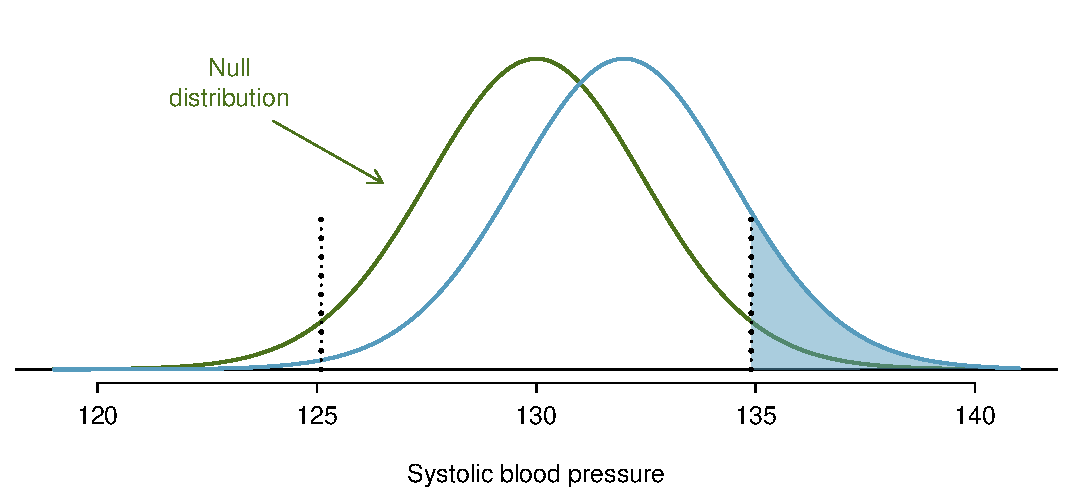
\includegraphics[width=\textwidth]{power/OneSampleIntroduction/power132And141/power132And141}
\caption{The sampling distribution of $\bar{x}$ under two scenarios. Left: $N(130, 2.5)$. Right: $N(132, 2.5)$, and the shaded area in this distribution represents the power of the test.}
\label{power132And141}
\end{figure}

The probability of rejecting the null hypothesis is called the \term{power}. The power varies depending on what we suppose the truth might be. In Example~\ref{computePowerIfMuIs132AndMu0Is130}, the difference between the null value and the supposed true mean was relatively small, so the power was also small: only 0.123. However, when the truth is far from the null value, where we use the standard error as a measure of what is far, the power tends to increase.

\begin{exercise}
Suppose the true sampling distribution of $\bar{x}$ is centered at 140. That is, $\bar{x}$ comes from $N(140, 2.5)$. What would the power be under this scenario? It may be helpful to draw $N(140, 2.5)$ and shade the area representing power on Figure~\ref{power132And141}; use the same cutoff values identified in Example~\ref{computePowerIfMuIs132AndMu0Is130}.\footnote{Draw the distribution $N(140, 2.5)$, then find the area above 134.9: about 0.979. If the true mean is 140, the power is about 0.979.}
\end{exercise}

\begin{exercise}
If the power of a test is 0.979 for a particular mean, what is the Type~2 Error rate for this mean?\footnote{The Type 2 Error rate represents the probability of failing to reject the null hypothesis. Since the power is the probability we do reject, the Type 2 Error rate will be $1-0.979 = 0.021$.}
\end{exercise}

\begin{exercise}
Provide an intuitive explanation for why we are more likely to reject $H_0$ when the true mean is further from the null value.\footnote{Answers may vary a little. When the truth is far from the null value, the point estimate also tends to be far from the null value, making it easier to detect the difference and reject $H_0$.}
\end{exercise}

\subsection{Statistical significance versus practical significance}

When the sample size becomes larger, point estimates become more precise and any real differences in the mean and null value become easier to detect and recognize. Even a very small difference would likely be detected if we took a large enough sample. Sometimes researchers will take such large samples that even the slightest difference is detected. While we still say that difference is \term{statistically significant}, it might not be \term{practically significant}.

Statistically significant differences are sometimes so minor that they are not practically relevant. This is especially important to research: if we conduct a study, we want to focus on finding a meaningful result. We don't want to spend lots of money finding results that hold no practical value.

The role of a statistician in conducting a study often includes planning the size of the study. The statistician might first consult experts or scientific literature to learn what would be the smallest meaningful difference from the null value. She also would obtain some reasonable estimate for the standard deviation. With these important pieces of information, she would choose a sufficiently large sample size so that the power for the meaningful difference is perhaps 80\% or 90\%. While larger sample sizes may still be used, she might advise against using them in some cases, such as when collecting more data than is truly necessary is unethical (e.g. a clinical trial) or where collecting the data is relatively costly.

%%

%_____
\pagebreak
\section*{Fitting models for nonlinear trends}

Prerequisites: Sections~1.1-1.6, 3.1, 4.1-4.4, 7.1-7.4, and~8.1 from \href{http://www.openintro.org/stat/textbook.php}{OpenIntro Statistics} are the bare minimum.

Figure~\ref{nonlinear} presents two examples of nonlinear relationships between two numerical variables. We'll introduce two techniques for fitting these two data sets: (1)~transforming the response variable and (2)~fitting nonlinear model using polynomial terms in multiple regression. While these two methods are very useful, there is no ``one size fits all'' modeling solution, and there are plenty of situations where these two methods will be insufficient for your needs. If you find that nonlinearity or challenges with residuals cannot be adequately addressed using these methods, consider turning to additional statistical methods.\footnote{See the \href{http://www.openintro.org/stat/supplements.php?feature=regression_online_extra_more_free_books}{Supplement page on openintro.org} for recommended free books that may be useful, or post a question on the online \href{http://www.openintro.org/stat/forums.php}{Public Forums on openintro.org}.}

\begin{figure}[h]
\centering
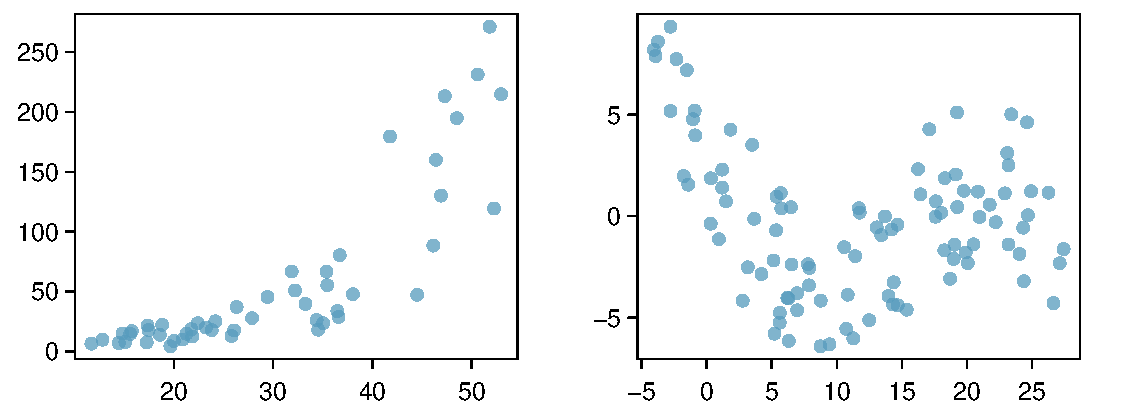
\includegraphics[width=\textwidth]{RegressionExtras/figures/nonlinear/nonlinear} 
\caption{Two pairs of numerical variables where each relationship is nonlinear. The residuals may also show other deviations that must be considered when modeling these data, including non-normal or \term{heteroskedastic} residuals (\emph{heteroskedastic} means \emph{non-constant variance}).}
\label{nonlinear}
\end{figure}

The techniques introduced in this section may be useful when the first, second, or fourth conditions for a simpler linear model are violated:
\begin{enumerate}
\setlength{\itemsep}{0mm}
\item the model residuals should be nearly normal,
\item the variability of the residuals is nearly constant,
\item the residuals are independent, and
\item each variable is linearly related to the outcome.
\end{enumerate}

\subsection{Transformations on the response}

Consider the scatterplot in the left panel of Figure~\ref{nonlinear}. Here, the response $y$ (vertical) tends to be positive but grow quickly. Additionally, the residuals show non-constant variance, because they are more variable for larger values of $x$ (horizontal) and $y$. These two characteristics of the untransformed data are a clue that a~transformation may be~useful.

In Section~1.6 of \href{http://www.openintro.org/stat/textbook.php}{OpenIntro Statistics}, we learned about the power of transformations to make skewed data more symmetric. If we look at a histogram of the $x$ and $y$ variables in Figure~\ref{nonlinear1-2}, we can see that $x$ shows a very slight right skew and $y$ is strongly right skewed. This suggests that it may be useful to transform the $y$ variable. Had $x$ been strongly right skewed, then we should have also considered using a transformation on $x$.

There are many possible transformations, but one of the most common is the natural log-transformation (sometimes written as $ln$). We'll take the natural log for the $y$ values and call this new variable~$y^\star$:
\begin{align*}
y^\star = \log y\text{, where ``log'' is the natural log}
\end{align*}
Figure~\ref{nonlinear1-3} shows $y^\star$ plotted against $x$. The data now show a linear relationship, where outliers are limited and the variability is roughly constant. Such an outcome is ideal, though far from guaranteed.

\begin{figure}
\centering
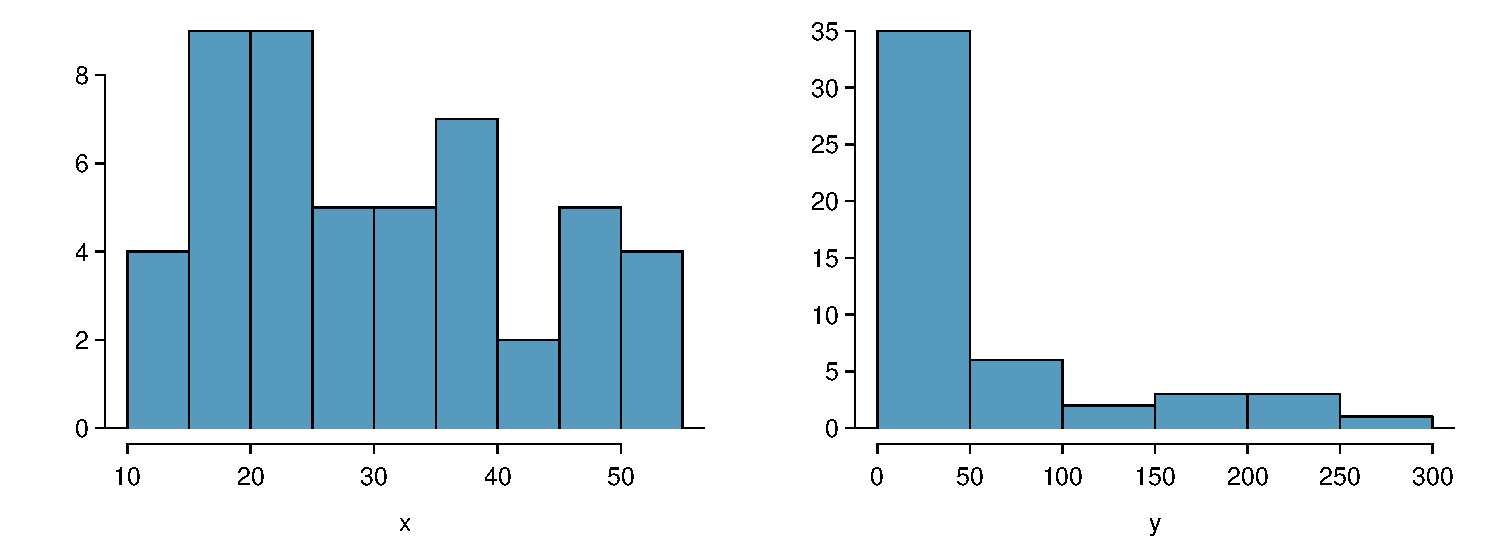
\includegraphics[width=\textwidth]{RegressionExtras/figures/nonlinear/nonlinear1-2}
\caption{Histograms for both the $x$ and $y$ variables from the left panel of Figure~\ref{nonlinear}.}
\label{nonlinear1-2}
\end{figure}

\begin{figure}
\centering
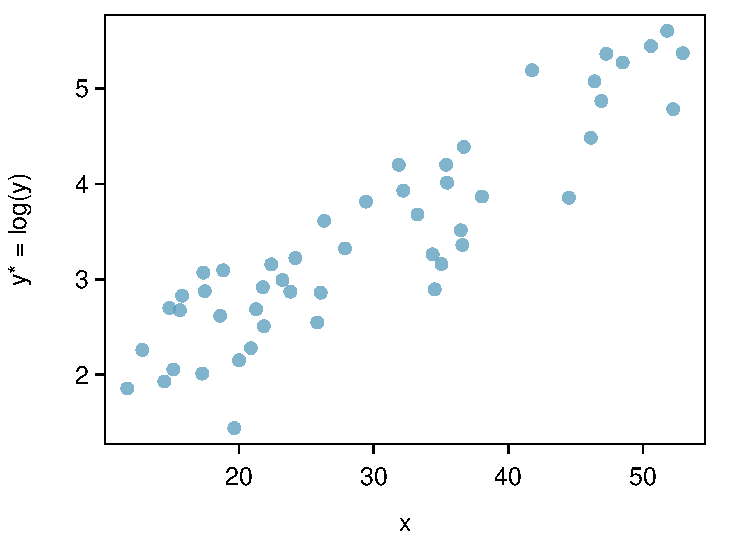
\includegraphics[width=0.7\textwidth]{RegressionExtras/figures/nonlinear/nonlinear1-3}
\caption{A plot of $y^\star$ (the result of transforming $y$ by taking the natural logarithm $\log y$) against $x$. The relationship between $y^\star$ and $x$ appears to be linear.}
\label{nonlinear1-3}
\end{figure}

We may now readily fit a linear model to the transformed scatterplot:
\begin{align*}
\hat{y}^\star &= 1.03 + 0.08x \\
y^\star &= 1.03 + 0.08x + residuals
\end{align*}
In the first equation above, the formula has been written in the form used by \href{http://www.openintro.org/stat/textbook.php}{OpenIntro Statistics}. The second line is a more general way to write this formula. This general form is important when we are transforming data since we often want to \term{back-transform} the data. Here, we back-transform by substituting $\log(y)$ for $y^\star$ and then solve for $y$:
\begin{align*}
y^\star &= 1.03 + 0.08x + residuals \\
\log(y) &= 1.03 + 0.08x + residuals \\
y &= e^{1.03 + 0.08x + residuals}
\end{align*}
In this way, we can now enter a value for $x$ and get an estimate for what value we think $y$ will take. This fitted line is shown in Figure~\ref{nonlinear1-4}.

\begin{figure}
\centering
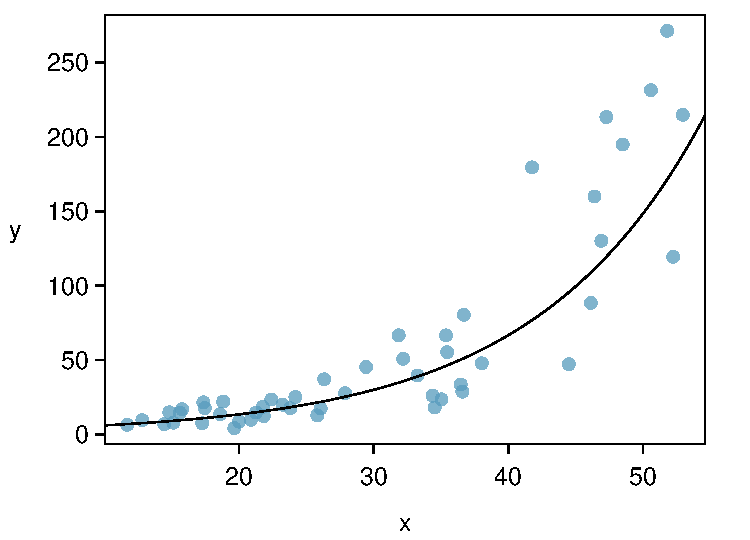
\includegraphics[width=0.7\textwidth]{RegressionExtras/figures/nonlinear/nonlinear1-4}
\caption{A nonlinear curve through the data generated by fitting a model of the form $\log y = \beta_0 + \beta_1x + residuals$, then solving for $y$.}
\label{nonlinear1-4}
\end{figure}

The predicted value for $y$ in this model should \emph{not} be confused with the expected (or mean) value of $y$ for a given value of $x$, though the result may be somewhat close. The footnote provides an explanation of the difference for the interested reader.\footnote{Suppose we collected many observations where $x=35$. This model suggests that the distribution of the corresponding $y$ values would be skewed as a result of the relationship between the residuals and the outcome $y$ being nonlinear. The model (roughly speaking) estimates the median for each value of $x$. Because the median is not the same as a mean in a skewed distribution, the model will not provide the expected value of $y$, though often times it will be close.}
%\begin{align*}
%\bar{y} &= e^{1.03 + 0.08x}\quad\text{(wrong!)} \\
%\end{align*}

\begin{tipBox}{\tipBoxTitle{Interpreting coefficients from a model that used $\log y$}
If the outcome in a model was transformed using the natural logarithm and the model fits well, then $y$ tends to grow (or decay) \term{exponentially} relative to $x$.} % For~example, in the model shown in Figure~\ref{nonlinear1-4}, a ``typical'' value for $y$ would be twice as large when $x$ is $\frac{\log2}{0.08} = 8.66$ units larger. If we compared the typical values for $y$ when $x=20$, $x=28.66$, and $x=37.32$, then $y_{x=28.66}$ would be twice as large as $y_{x=20}$, and $y_{x=37.32}$ would be \emph{four} times as large as $y_{x=20}$.}
\end{tipBox}

\begin{caution}{Transformations can be abused}
{There is a very large number of possible transformations. If we keep trying transformations until one ``works'', we have not effectively modeled our data. Rather, we have performed a complicated form of data fishing where we mine the data until we see structure. This apparent structure may just be due to chance. Therefore, think carefully about transformations before applying them.}
\end{caution}

You are once again armed with knowledge that is both powerful and dangerous. This very brief introduction to transformations should be useful for informal projects. For a more complete review of this topic, visit Chapter~8 of \emph{Practical Regression and ANOVA~in~R}, which can be found in the Free Books section on the \href{http://www.openintro.org/stat/supplements.php?feature=regression_online_extra_more_free_books}{Supplements page of openintro.org}.


\subsection{Fitting a polynomial curve}
\label{fittingAPolynomialCurve}

%A second strategy for addressing nonlinearity is to create new variables using existing variables fit a new set of variables, ones that themselves try to match the nonlinearity of the outcome $y$. It is common to try to add additional polynomial terms to the model. In effect, we generate a new set of variables $x_2=x^2$, $x_3=x^3$, and so one that we can consider adding to the model (note: we rarely use $x_3=x^3$ and beyond, though we will encounter such an example in this section).

Let's take a look at the second nonlinear relationship we saw in Figure~\ref{nonlinear}, which appears again in Figure~\ref{nonlinear2-2} with a poorly-fit straight line. Here we see what appears to be a nonlinear relationship but where the residuals would be approximately \term{homoskedastic} (constant variance) if we could reasonably model the curve of the line. This is a good signal that we want to fit a curve but not perform a transformation. We can do so by generating a \term{polynomial basis} of $x$: $x_1=x$, $x_2 = x^2$, $x_3 = x^3$, and so on. In short, we will use the variables $x_1$, $x_2$, $x_3$, ... in a multiple regression model instead of simply the original variable $x$. We should note that it is uncommon to use terms beyond $x_2 = x^2$ and very rarely beyond $x_3=x^3$.

We start by fitting a linear model to the data, where the best-fitting straight line is shown in Figure~\ref{nonlinear2-2} and summarized as
\begin{align*}
y = 0.8441 - 0.0964x + residuals
\end{align*}
Even without checking the residual plot, it is evident that this line does not fit the data well, though Table~\ref{nonlinear2-linearfitsummary} shows that the linear term is statistically significant.

\begin{figure}
\centering
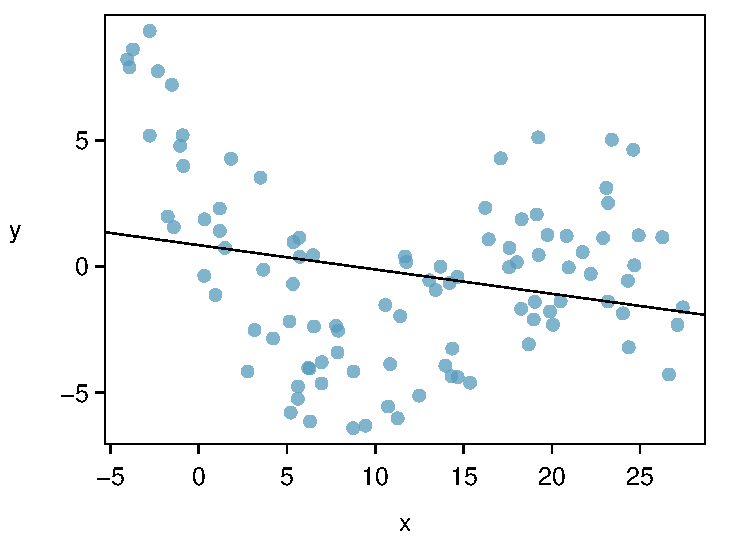
\includegraphics[width=0.6\textwidth]{RegressionExtras/figures/nonlinear/nonlinear2-2}
\caption{Scatterplot with the best-fitting straight line, which does not fit the data well.}
\label{nonlinear2-2}
\end{figure}

\begin{exercise}
Suppose you were providing feedback to someone on a project, and the colleague had fit the line to the data shown in Figure~\ref{nonlinear2-2}. Suppose also that your colleague believes this model is sufficient because the estimate for the slope is statistically significant. Explain why the model is inappropriate. One possible explanation is provided in the footnote.\footnote{Regression models require certain conditions to be met. In particular, the residuals must be independent of each other. However, when we look at the residuals from the fit in Figure~\ref{nonlinear2-2}, there is a clear trend in the residuals not captured by the straight line, meaning the independence condition is violated and the model is inadequate.}
\end{exercise}

\begin{table}
\centering
\begin{tabular}{rrrrr}
  \hline
 & Estimate & Std. Error & t value & Pr($>$$|$t$|$) \\ 
  \hline
(Intercept) & 0.8441 & 0.5799 & 1.46 & 0.1487 \\ 
  x1  & -0.0964 & 0.0397 & -2.43 & 0.0169 \\ 
   \hline
\end{tabular}
\caption{Summary for a straight line fit to the data shown in Figure~\ref{nonlinear2-2}.}
\label{nonlinear2-linearfitsummary}
\end{table}

As a next step, we'll add another variable to the model: $x_2=x^2$. This new variable is itself a transformation on the variable $x$. However, rather than substituting $x_2$ for $x$, we'll fit a multiple regression model \emph{including both variables} from the polynomial basis:
\begin{align*}
y = \beta_0 + \beta_1x_1 + \beta_2x_2 + residuals
\end{align*}
The best-fitting model of this form is shown in Figure~\ref{nonlinear2-3}, and the summary for the model is shown in Table~\ref{nonlinear2-quadfitsummary}.

\begin{figure}
\centering
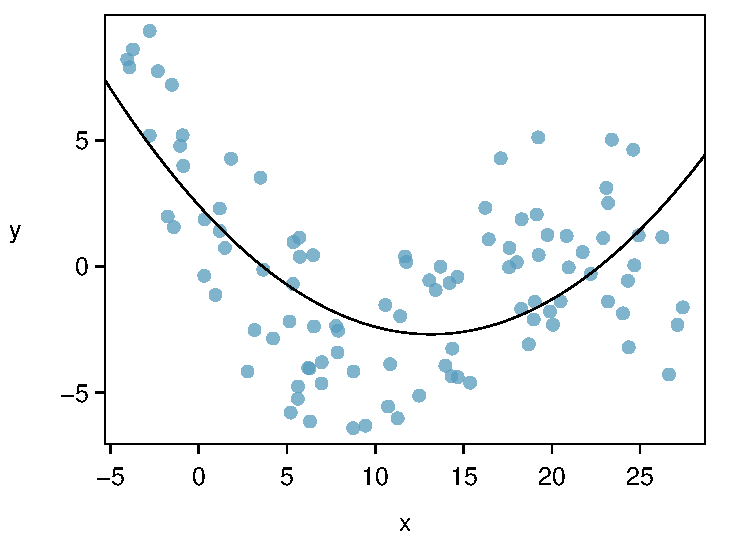
\includegraphics[width=0.65\textwidth]{RegressionExtras/figures/nonlinear/nonlinear2-3}
\caption{Scatterplot with the best-fitting quadratic line, which fits better than a straight-line but still misses some data structures. For example, the model underestimates much of the data for the range -5 to 0 and it overestimates nearly all of the data between 5 and 10.}
\label{nonlinear2-3}
\end{figure}

\begin{table}
\centering
\begin{tabular}{rrrrr}
  \hline
 & Estimate & Std. Error & t value & Pr($>$$|$t$|$) \\ 
  \hline
(Intercept) & 2.4252 & 0.5079 & 4.78 & 0.0000 \\ 
  x1  & -0.7769 & 0.0956 & -8.13 & 0.0000 \\ 
  x2  & 0.0295 & 0.0039 & 7.55 & 0.0000 \\ 
   \hline
\end{tabular}
\caption{Summary for a quadratic fit to the data shown in Figure~\ref{nonlinear2-3}.}
\label{nonlinear2-quadfitsummary}
\end{table}

\begin{example}{Write out the best fitting quadratic model using Table~\ref{nonlinear2-quadfitsummary}.}
The model may be written as
\begin{align*}
y &= 2.4252 - 0.7769x_1 + 0.0295x_2 + residuals \\
	&= 2.4252 - 0.7769x + 0.0295x^2 + residuals
\end{align*}
\end{example}

In this example a quadratic model is still insufficient, so we will try a cubic polynomial (also known as a third-order polynomial). We will try fitting a model based on a cubic polynomial:
\begin{align*}
y &= \beta_0 + \beta_1x_1 + \beta_2x_2 + \beta_3x_3 + residuals \\
	&= \beta_0 + \beta_1x + \beta_2x^2 + \beta_3x^3 + residuals
\end{align*}
Such a model is summarized in Figure~\ref{nonlinear2-4} and Table~\ref{nonlinear2-cubicfitsummary}.
\begin{figure}
\centering
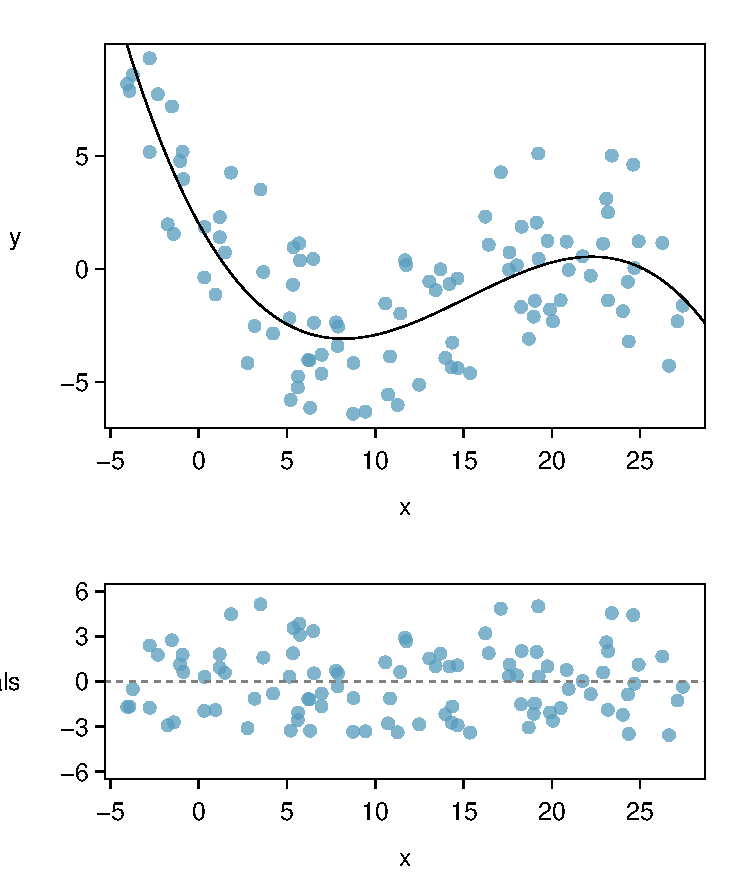
\includegraphics[width=0.65\textwidth]{RegressionExtras/figures/nonlinear/nonlinear2-4}
\caption{Scatterplot with the best-fitting cubic line. The residual plot shows no apparent structure, which is a good sign the model is fitting well.}
\label{nonlinear2-4}
\end{figure}
\begin{table}
\centering
\begin{tabular}{rrrrr}
  \hline
 & Estimate & Std. Error & t value & Pr($>$$|$t$|$) \\ 
  \hline
(Intercept) & 2.0187 & 0.4242 & 4.76 & 0.0000 \\ 
  x1 & -1.4202 & 0.1236 & -11.49 & 0.0000 \\ 
  x2 & 0.1187 & 0.0136 & 8.75 & 0.0000 \\ 
  x3 & -0.0026 & 0.0004 & -6.77 & 0.0000 \\ 
   \hline
\end{tabular}
\caption{Summary for a cubic line fit to the data shown in Figure~\ref{nonlinear2-4}}
\label{nonlinear2-cubicfitsummary}
\end{table}

\begin{exercise}
Write out the best fitting quadratic model using Table~\ref{nonlinear2-cubicfitsummary}. The solution is in the footnote.\footnote{$y = 2.0187 - 1.4202x_1 + 0.1187x_2 - 0.0026x_3 + residuals = 2.0187 - 1.4202x + 0.1187x^2 - 0.0026x^3 + residuals$}
\end{exercise}

The initial prognosis from the residual plot is that the cubic model fits very well. However, a complete analysis would include checking the model diagnostics carefully, which is a topic discussed in Section~8.3 of \href{http://www.openintro.org/stat/textbook.php}{OpenIntro Statistics}.

\begin{tipBox}{\tipBoxTitle{Stick with lower-order polynomials}
If you want to try out using a polynomial term in your model, consider $x^2$ and perhaps $x^3$ if the model is still not a good fit. If a cubic polynomial will not model your data well, then be very cautious about trying higher-order polynomials. Instead, consider learning about regression splines, kernel smoothing, or some other statistical technique. See the textbook \href{http://www.openintro.org/stat/supplements.php?feature=regression_online_extra_more_free_books}{Elements of Statistical Learning} for more information on advanced modeling techniques.}
\end{tipBox} 

\begin{caution}{Do not extrapolate with transformed models or models that use polynomial terms}
{Extrapolation is already treacherous for any model, but it can be much worse for transformed data or data that includes polynomial terms, as the model can deviate very rapidly from the typical values observed in the original data set.}
\end{caution}


































%
%\noindent This document provides a foundation of concepts for using interaction terms in regression.  \\








%_____
\pagebreak
\section*{Interaction terms}

Prerequisites: Sections~1.1-1.6, 3.1, 4.1-4.4, 7.1-7.4, and~8.1 from \href{http://www.openintro.org/stat/textbook.php}{OpenIntro Statistics} are the bare minimum.

\begin{example}{Suppose we were to conduct an experiment where we measured the effect of water and sunlight on plant growth. While each of these contributes individually to plant growth, we might wonder whether there is any interaction between them when promoting growth.}
First and foremost, we would notice no amount of water is sufficient for plant growth if sunshine is completely absent, and vice versa. If you modeled growth simply as a function of sunshine plus water (for example, using a basic multiple regression model introduced in Chapter~8 of \href{http://www.openintro.org/stat/textbook.php}{OpenIntro Statistics}), you'd run into trouble at first. This section tackles this challenge through the use of interaction terms in the context of multiple regression.
\end{example}

Let's consider an experiment that examines the impact of Vitamin C from two sources on the growth of teeth in Guinea pigs.\footnote{Bliss CI. 1952. The Statistics of Bioassay. \emph{Academic Press}. We'll consider a subset of the data available (excludes dose level 0.5), which can be accessed in R via the \data{ToothGrowth} data set.} In this experiment, each Guinea pig was randomly assigned to one of two possible levels of each variable:
\begin{itemize}
\setlength{\itemsep}{0mm}
\item \var{supp} indicates a supplement type for Vitamin C, with levels \resp{VC} for ascorbic acid and \resp{OJ} for orange juice.
\item \var{dose} indicates the amount of Vitamin C, which takes values of either 1~or~2~mg.
\end{itemize}
The researchers measured the length of the teeth of the Guinea pigs as the experimental outcome. The data are summarized in Figure~\ref{interaction}, where each combination of treatments was applied to 10 Guinea pigs.

\begin{figure}[h]
\centering
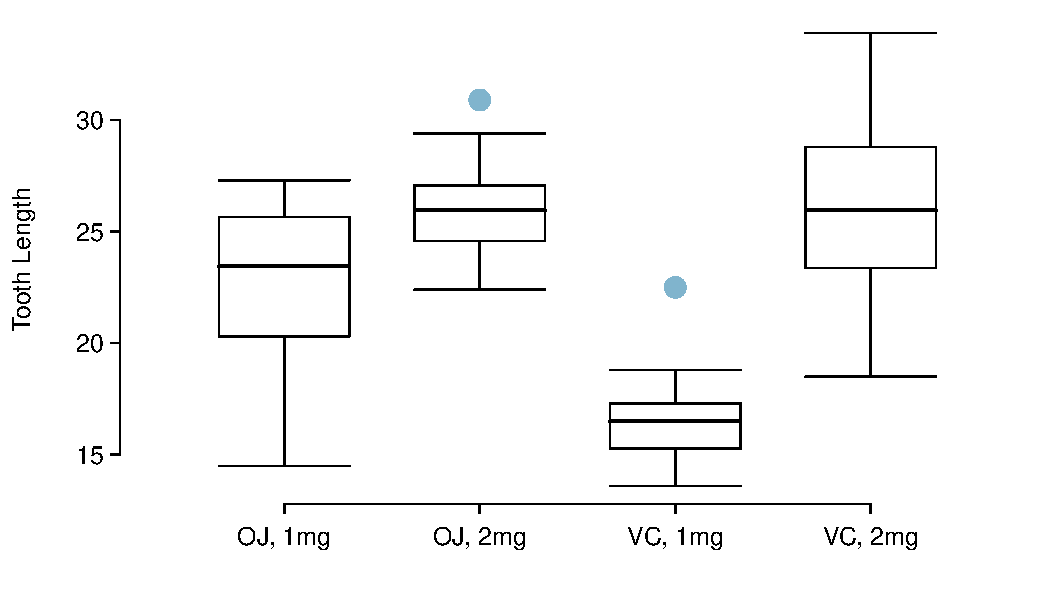
\includegraphics[width=0.9\textwidth]{RegressionExtras/figures/interaction/interaction}
\caption{Side-by-side box plots summarizing the \data{ToothGrowth} data set. Each Guinea pig received a specific amount of Vitamin C (1mg or 2mg) and the source of that Vitamin C was either ascorbic acid (\resp{VC}) or orange juice (\resp{OJ}).}
\label{interaction}
\end{figure}

\begin{tipBox}{\tipBoxTitle{Experiments can randomize along 1 \emph{or more} variables}
In OpenIntro Statistics, we only considered experiments where the researchers randomly assigned one type of treatment. However, by randomizing more treatments, we can identify causal relationships among a set of variables. The example in this section takes a small step into the field of statistics called \term{experimental design}.}
\end{tipBox}



Our aim is to build a multiple regression model that accurately estimates the impact of each variable. We will start by building a model of the following form:
\begin{align*}
y = \beta_0 + \beta_{supp}x_{supp} + \beta_{dose}x_{dose} + residuals
\end{align*}
The fitted model is summarized in Table~\ref{interaction-simpleModelSummary}. Notice the slightly different variable name \var{suppVC} in the table (rather than \var{supp}). This new \var{suppVC} variable was automatically generated by the statistical software since \var{supp} was a categorical variable. The new variable takes value 1 when the supplement is \resp{VC} and 0 when the supplement is \resp{OJ}.
\begin{table}
\centering
\begin{tabular}{rrrrr}
  \hline
 & Estimate & Std. Error & t value & Pr($>$$|$t$|$) \\ 
  \hline
(Intercept) & 14.8325 & 2.0319 & 7.30 & 0.0000 \\ 
  suppVC & -2.9250 & 1.2253 & -2.39 & 0.0222 \\ 
  dose & 6.3650 & 1.2253 & 5.19 & 0.0000 \\ 
   \hline
\end{tabular}
\caption{Summary for the multiple regression model for the Guinea pig experiment.}
\label{interaction-simpleModelSummary}
\end{table}

\begin{exercise}\label{writeOutInteractionModelWOInteraction}
Write the model represented by the output shown in Table~\ref{interaction-simpleModelSummary}. The solution is in the footnote.\footnote{$y = 14.83 - 2.93x_{suppVC} + 6.37x_{dose} + residuals$}
\end{exercise}

\begin{exercise}\label{findInteractionNeeded}
Use the model from Exercise~\ref{writeOutInteractionModelWOInteraction} to predict an outcome for each possible combination of variables. Calculate these means and plot them on Figure~\ref{interaction}. The~plot is provided in the footnote.\footnote{The means are represented by red dotted lines.\\\color{white}WWW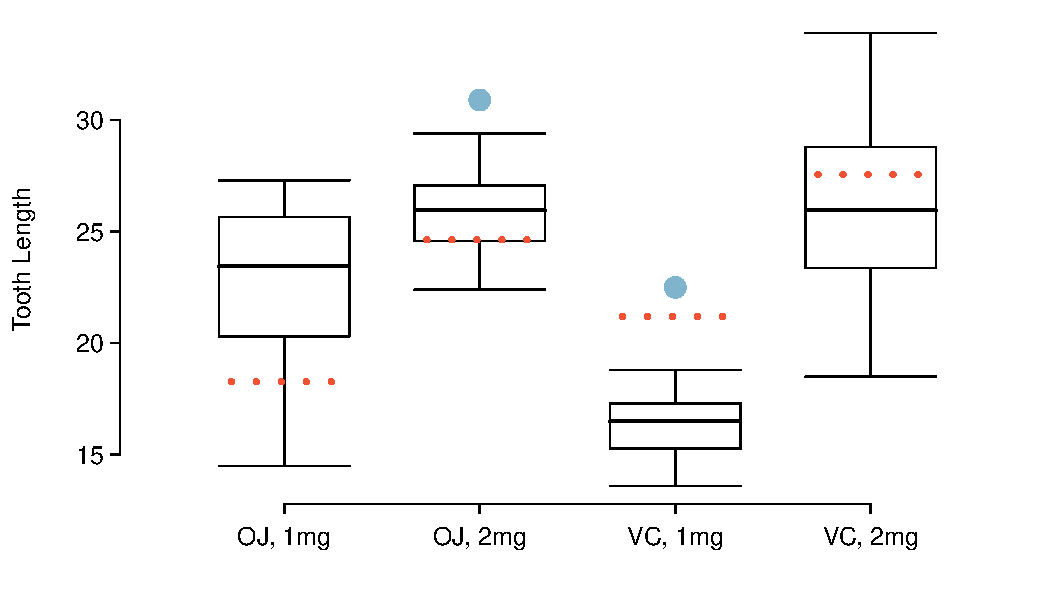
\includegraphics[width=0.7\textwidth]{RegressionExtras/figures/interaction/interaction-noint-w-mean}}
\end{exercise}

Re-examining the solution to Exercise~\ref{findInteractionNeeded}, the fitted values fall far from the centers of the groups, which is a signal that the model does not fit the data very well.

The model you identified in Exercise~\ref{writeOutInteractionModelWOInteraction} assumes that the effects of the supplement and dose are independent. However, it is also possible that the two treatments interact, i.e. the effect of one may partially depend on the value of the other. We can model this \term{interaction} effect using a new term:
\begin{align*}
y = \beta_0 + \beta_{suppVC}x_{suppVC} + \beta_{dose}x_{dose} + \beta_{suppVC:dose}x_{suppVC}x_{dose} + residuals
\end{align*}
The term $\beta_{suppVC:dose}x_{suppVC}x_{dose}$ represents the interaction. The summary for this model is shown in Table~\ref{modelSummaryIncludingInteraction}, and the interaction term is indeed statistically significant.
\begin{table}[ht]
\centering
\begin{tabular}{rrrrr}
  \hline
 & Estimate & Std. Error & t value & Pr($>$$|$t$|$) \\ 
  \hline
(Intercept) & 19.3400 & 2.5419 & 7.61 & 0.0000 \\ 
  suppVC & -11.9400 & 3.5948 & -3.32 & 0.0021 \\ 
  dose & 3.3600 & 1.6076 & 2.09 & 0.0437 \\ 
  suppVC:dose & 6.0100 & 2.2735 & 2.64 & 0.0121 \\ 
   \hline
\end{tabular}
\caption{Summary for the multiple regression model with the interaction term.}
\label{modelSummaryIncludingInteraction}
\end{table}

\begin{exercise} \label{identifyModelWInteraction}
Write the model summarized by Table~\ref{modelSummaryIncludingInteraction}. The solution is in the footnote.\footnote{$y = 19.34  - 11.94x_{suppVC} + 3.36 x_{dose} + 6.01 x_{suppVC}x_{dose} + residuals$ (could also use $x_{suppVC:dose}$ in place of $x_{suppVC}x_{dose}$).}
\end{exercise}

\begin{exercise} \label{CalculatedPredictedMeans}
Using the model equation you generated in Exercise~\ref{identifyModelWInteraction}, calculate the predicted value for a new observation for each group. The solution is in the footnote.\footnote{Consider the predicted value for $y$ under each of the four possible supplement/dose scenarios:
\begin{itemize}
\setlength{\itemsep}{0mm}
\item Orange juice and dosage of 1mg ($x_{suppVC}=0, x_{dose}=1$)
	\begin{align*}
	\hat{y} &= \beta_0 + \beta_{suppVC}x_{suppVC} +
			\beta_{dose}x_{dose} +
			\beta_{suppVC:dose}x_{suppVC}x_{dose} \\
		&= \beta_0 + \beta_{suppVC}\times 0 +
			\beta_{dose}\times 1 +
			\beta_{suppVC:dose}\times 0\times 1 \\
		&= \beta_0 + \beta_{dose}
		\sim b_0 + b_{dose}
		= 22.70
	\end{align*}
\item Orange juice and dosage of 2mg ($x_{suppVC}=0, x_{dose}=2$)
	\begin{align*}
	\hat{y} &= \beta_0 + \beta_{suppVC}x_{suppVC} +
			\beta_{dose}x_{dose} +
			\beta_{suppVC:dose}x_{suppVC}x_{dose} \\
		&= \beta_0 + \beta_{suppVC}\times 0 +
			\beta_{dose}\times 2 +
			\beta_{suppVC:dose}\times 0\times 2 \\
		&= \beta_0 + 2\beta_{dose}
		= b_0 + 2b_{dose}
		= 26.06
	\end{align*}
\item Ascorbic acide and dosage of 1mg ($x_{suppVC}=1, x_{dose}=1$)
	\begin{align*}
	\hat{y} &= \beta_0 + \beta_{suppVC}x_{suppVC} +
			\beta_{dose}x_{dose} +
			\beta_{suppVC:dose}x_{suppVC}x_{dose} \\
		&= \beta_0 + \beta_{suppVC}\times 1 +
			\beta_{dose}\times 1 +
			\beta_{suppVC:dose}\times 1\times 1 \\
		&= \beta_0 + \beta_{suppVC} + \beta_{dose} +
			\beta_{suppVC:dose}
		= b_0 + b_{suppVC} + b_{dose} +
			b_{suppVC:dose}
		= 16.77
	\end{align*}
\item Ascorbic acide and dosage of 2mg ($x_{suppVC}=1, x_{dose}=2$)
	\begin{align*}
	\hat{y} &= \beta_0 + \beta_{suppVC}x_{suppVC} +
			\beta_{dose}x_{dose} +
			\beta_{suppVC:dose}x_{suppVC}x_{dose} \\
		&= \beta_0 + \beta_{suppVC}\times 1 +
			\beta_{dose}\times 2 +
			\beta_{suppVC:dose}\times 1\times 2 \\
		&= \beta_0 + \beta_{suppVC} + 2\beta_{dose} +
			2\beta_{suppVC:dose}
		= b_0 + b_{suppVC} + 2b_{dose} +
			2b_{suppVC:dose}
		= 26.14
	\end{align*}
\end{itemize}}
\end{exercise}

%A sharp eye will notice that the means calculated in Exercise~\ref{CalculatedPredictedMeans} are the same means for each of the four possible treatment combinations. The model with the interaction can fully adjust for differences among the groups, and since the best guess at a future value is the mean, the model calculates the best estimates of the $\beta_i$ terms using the group means.







\pagebreak

\begin{exercise}
Suppose we were to run an experiment where 24 bean plants are randomized into one of four groups:
\begin{itemize}
\setlength{\itemsep}{0mm}
\item Each plant receives 1~teaspoon of water and 1~hour of sunlight each~day.
\item Each plant receives 4~tablespoons of water and 1~hour of sunlight each~day.
\item Each plant receives 1~teaspoon of water and 8~hours of sunlight each~day.
\item Each plant receives 4~tablespoons of water and 8~hours of sunlight each~day.
\end{itemize}
\begin{enumerate}[(a)]
\item Which group do you think will have the least plant growth?
\item The most plant growth?
\item How confident are you in your answers?
\item Do you think the effects of the water and sunlight on plans are independent? If so, explain why. If not, explain how you might model this relationship.
\end{enumerate}
\end{exercise}





%_____
%\pagebreak
%\section{Prediction of the mean response}



%_____
%\pagebreak
%\section{Prediction of future values}

%Note the extreme importance of the normality assumption regarding the residuals.



















































\end{document}  